%!TEX root = practicum3.tex
\subsection*{Point in Triangle}

% Theory
We try to determine if the point \vec{Q} lies in the triangle defined by the points $\vec{P_1}$, $\vec{P_2}$ and $\vec{P_3}$. To this end we define the vectors $\vec{v}_1 = \vec{P_2} - \vec{P_1}$ and $\vec{v_2} = \vec{P_3} - \vec{P_1}$, see \autoref{fig:a:triangle_point}. Each point $\vec{P}$ inside the grey area in this figure can be described as:
\begin{equation} \label{eq:a:trianglePointEquation}
	\vec{P} = \vec{P_1} + a \cdot \vec{v_1} + b \cdot \vec{v_2}.
\end{equation}

\begin{figure}
	\centering
	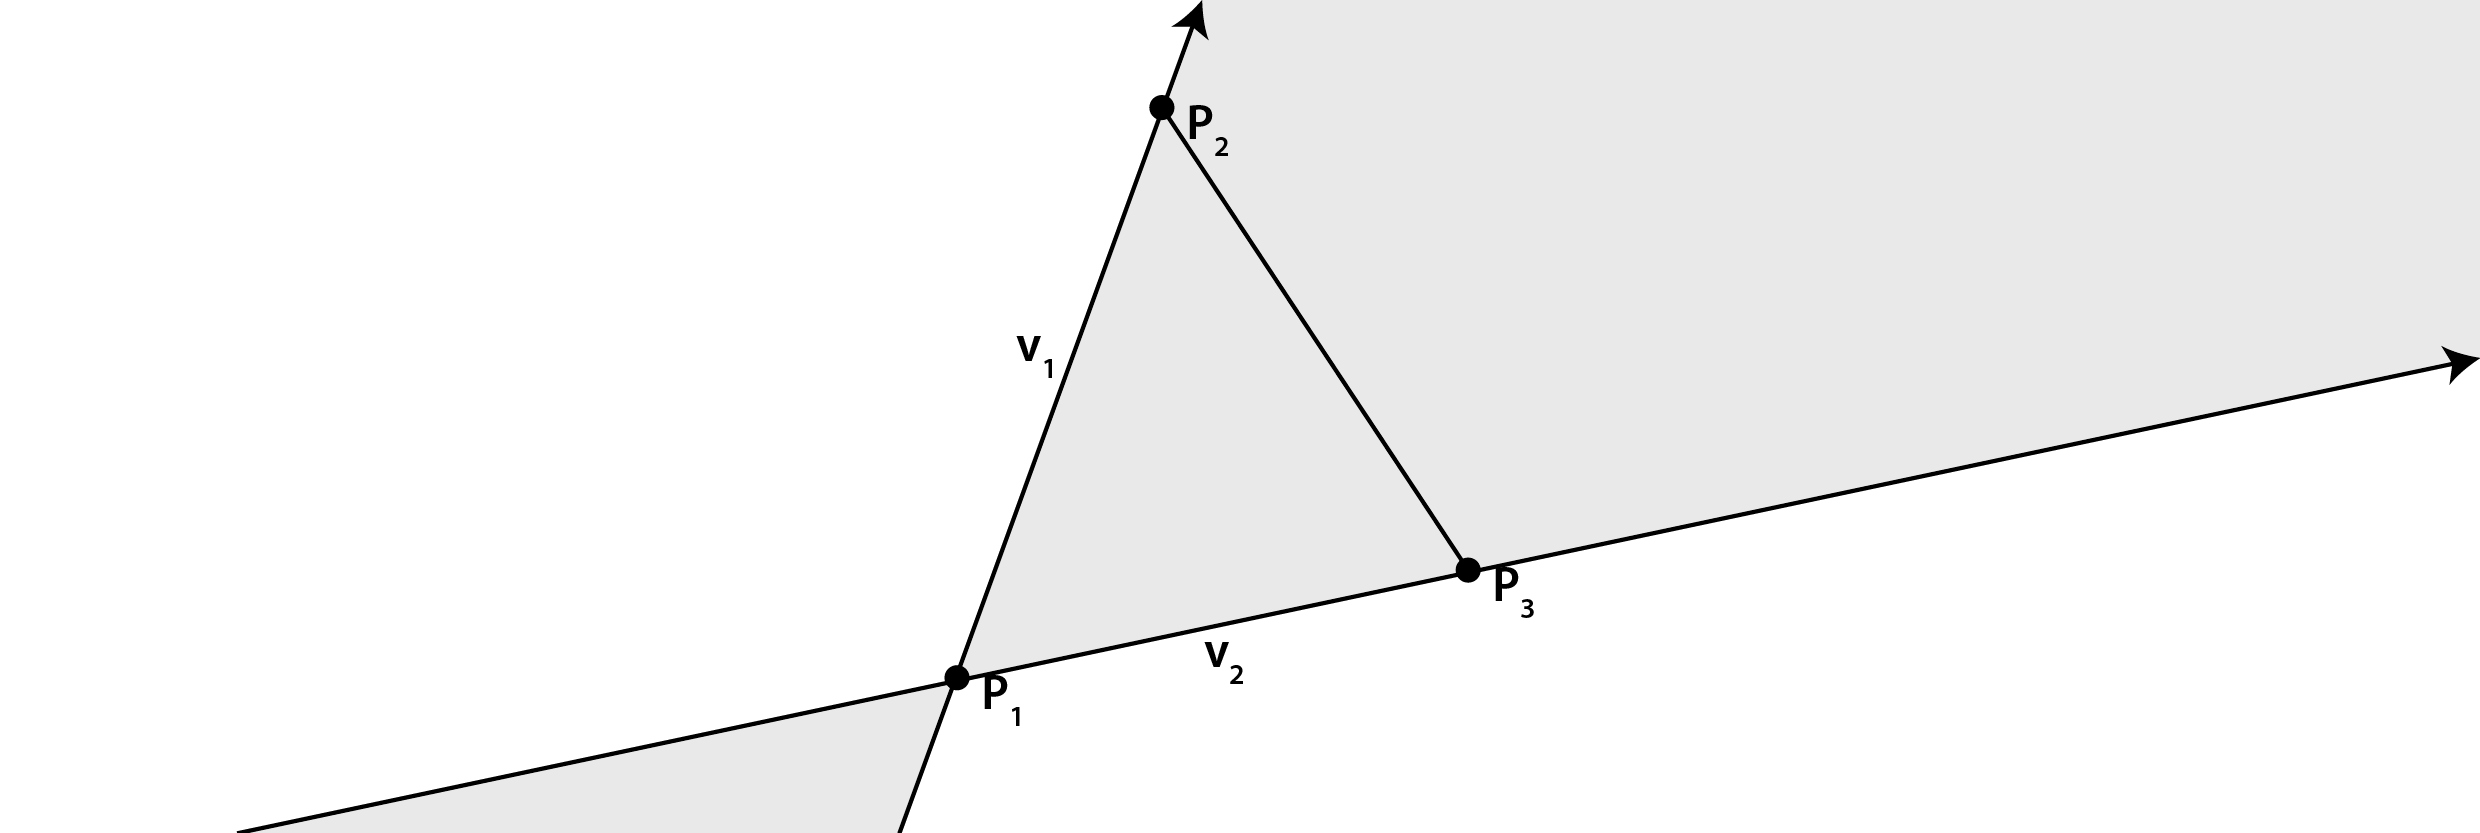
\includegraphics[width=0.9\textwidth, frame]{./img/a_triangle_point-01}
	\caption{A triangle defined by the points $\vec{P_1}$, $\vec{P_2}$ and $\vec{P_3}$, with the vectors $\vec{v_1}$ and $\vec{v_2}$. The grey area covers all points that can be described according to \eqref{eq:a:trianglePointEquation}.}
	\label{fig:a:triangle_point}
\end{figure}

For all points to the right of \vec{P_1} $a > 0$ and $b > 0$. The points that define the triangle can all be expressed according to \eqref{eq:a:trianglePointEquation}:
\begin{align}
	\vec{P_1} &= \vec{P_1} + 0 \cdot \vec{v_1} + 0 \cdot \vec{v_2} \label{eq:a:p1}\\ 
	\vec{P_2} &= \vec{P_1} + 1 \cdot \vec{v_1} + 0 \cdot \vec{v_2} \label{eq:a:p2}\\ 
	\vec{P_3} &= \vec{P_1} + 0 \cdot \vec{v_1} + 1 \cdot \vec{v_2} \label{eq:a:p3}.
\end{align}
If $a + b == 1$ the point lies on the edge between $\vec{P_2}$ and $\vec{P_3}$. Based on \autoref{eq:a:p1} through \ref{eq:a:p3} we find that a point \vec{Q} lies on the triangle if it can be expressed according to \eqref{eq:a:trianglePointEquation} with $a,b \in (0,1)$ and with $a + b < 1$. 

	\begin{lstlisting}[float, language=Mathematica, label={lst:a:pointInTriangleMathematica}, caption={Mathematica code used to compute the to compute $a$ and $b$.}]
p1 = {p10, p11};
p2 = {p20, p21};
p3 = {p30, p31};
v1 = p2 - p1;
v2 = p3 - p1;

p4 = p1 + a * v1 + b * v2;
p41 = Part[p4, 1] == Q0;
p42 = Part[p4, 2] == Q1;
solution = Solve[{p41, p42}, {a, b}]\end{lstlisting}

Solving the resulting equation with Mathematica, see \autoref{lst:a:pointInTriangleMathematica}, gives us expressions for $a$ and $b$, namely:
	\begin{align}
	a &= -\frac{-\vec{P_{1,0}} \vec{P_{3,1}}+\vec{P_{1,0}} \vec{Q1}+\vec{P_{1,1}} \vec{P_{3,0}}-\vec{P_{1,1}}
   \vec{Q_0} - \vec{P_{3,0}} \cdot \vec{Q_1}+\vec{P_{3,1}} \cdot \vec{Q_0}}{ - \vec{P_{1,0}}
   \vec{P_{2,1}}+\vec{P_{1,0}} \cdot \vec{P_{3,1}}+\vec{P_{1,1}} \cdot \vec{P_{20}} - \vec{P_{1,1}}
   \vec{P_{3,0}} - \vec{P_{2,0}} \cdot \vec{P_{3,1}}+\vec{P_{2,1}} \cdot \vec{P_{3,0}}}\label{eq:a:a}\\
	b &=  - \frac{ - \vec{P_{1,0}} \cdot \vec{P_{2,1}}+\vec{P_{1,0}} \cdot \vec{Q_1}+\vec{P_{1,1}} \cdot \vec{P_{2,0}} - \vec{P_{1,1}}
   \vec{Q_0} - \vec{P_{2,0}} \cdot \vec{Q_1}+\vec{P_{2,1}} \cdot \vec{Q_0}}{\vec{P_{1,0}}
   \vec{P_{2,1}} - \vec{P_{1,0}} \cdot \vec{P_{3,1}} - \vec{P_{1,1}} \cdot \vec{P_{2,0}}+\vec{P_{1,1}}
   \vec{P_{3,0}}+\vec{P_{2,0}} \cdot \vec{P_{3,1}} - \vec{P_{2,1}} \cdot \vec{P_{3,0}}}\label{eq:a:b}
	\end{align}
where \vec{P_{r,s}} represents the $s$'th element of the point $r$ and \vec{Q_t} represent the $t$'th element of the point \vec{Q}.

The denominator of \eqref{eq:a:a} and \eqref{eq:a:b} are the same, this is the magnitude of $\vec{v_1} \times \vec{v_2}$ where the vectors are made three-dimensional by adding a $z$-coordinate of zero, If that cross product is zero \vec{v_1} and \vec{v_2} are parallel and \eqref{eq:a:trianglePointEquation} can thus be only used to represent points on a line parallel to $\vec{v_1}$ and through $\vec{P_1}$. \\

% Implementatie
The method presented above is implemented in the method \t{point_in_triangle()} in the module \t{triangle}, see \autoref{lst:a:pointInTriangle}.

\lstinputlisting[float, firstline=5, lastline=32, label={lst:a:pointInTriangle}, caption={The method \t{point_in_triangle()} in the module \t{triangle}.}]{../triangle.py}

\subsection*{Finding the Triangle Containing the Point}
We have simply checked for all triangles that result from the triangulation if the point lies inside that triangle, see \autoref{lst:a:findContainingTriangle} for the method \t{find_containing_triangle()}. \autoref{fig:a:triangulationWithPoint} shows the triangulation of 100 points generated randomly with the seed set to 505. The triangle that contains the point \t{lp} (305, 350) is shown in green, as is the point it self. The containing triangle is defined by the points: (\num{434.746175446}, \num{275.228689898}), (\num{292.651351959}, \num{371.369188947}), (\num{335.384364149}, \num{245.801849268}).

The method \t{find_containing_triangle} is passed the global parameter \t{lp}, \t{triPts}, \t{xl} and \t{yl}, so that it may be reused for assignment C.

\begin{figure}
	\centering
	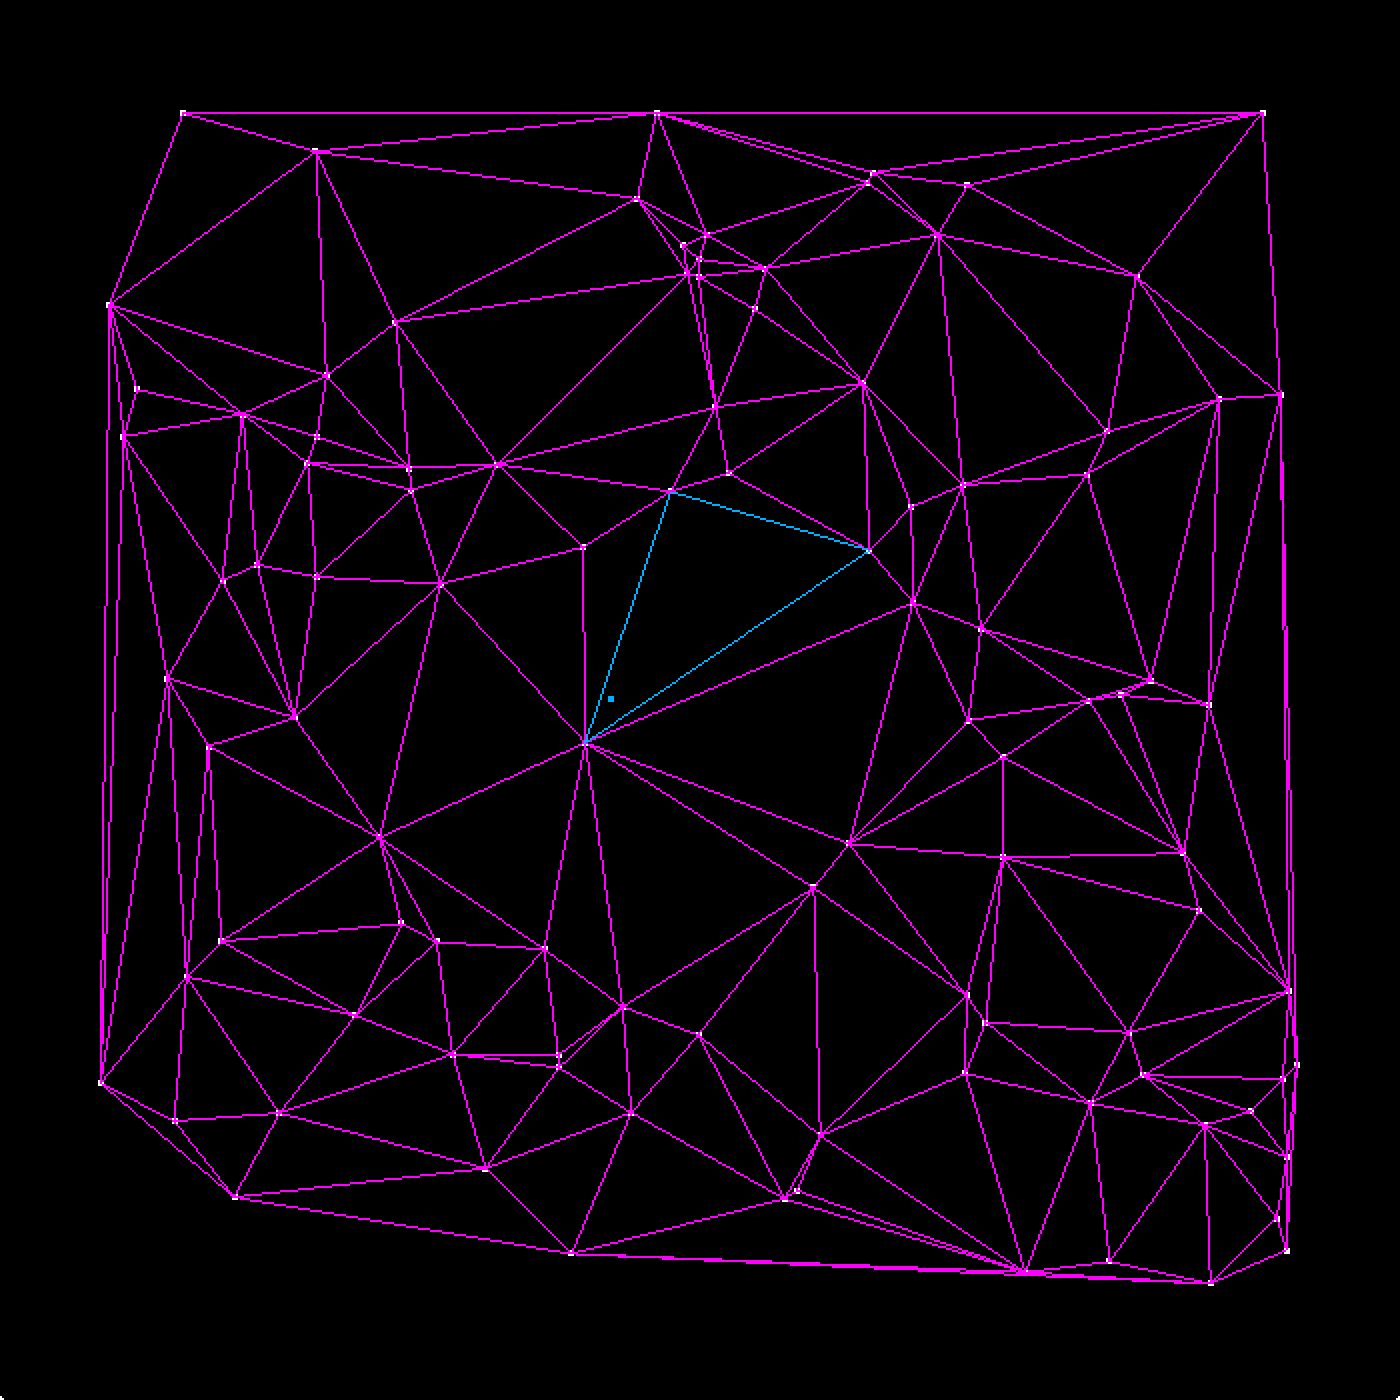
\includegraphics[width=0.5\textwidth]{./img/a_triangulationWithPoint}
	\caption{The triangulation of one hundred points, the triangle shown in green contains the point \t{lp}, also shown in green.}
	\label{fig:a:triangulationWithPoint}
\end{figure}

\lstinputlisting[float, firstline=143, lastline=171, label={lst:a:findContainingTriangle}, caption={The method \t{find_containing_triangle()}.}]{../assignment3A.py}
